\chapter{\hspace*{3pt} Experiments and Results}
\label{chapter:experiments}

Esse capítulo descreve os experimentos computacionais e os testes 

\section{\hspace*{3pt} Proof of Concept - Q\&A Communities}
\label{section:proof-of-concept}

The first evaluation of our approach is a proof of concept aiming to analyze the classification based on our method in posts of  Q\&A (Question and Answers) communities. 

Q\&A (Question and Answers) have emerged in the past few years as Web 2.0 becomes popular. They provide a place for users to ask specific questions and receive direct answers. 
The users exchange and share their knowledge explicitly by asking or answering questions in a set of predefined topics and categories. 

The volume of questions answered on Q\&A site so far exceeds the number of questions answered by library reference services \cite{Shah:2010} . As a result,  question and answer archives are numerous knowledge repositories \cite{Andrzejewski:2009}.


In this context, Stack Exchange\footnote{\url{https://stackexchange.com/}}
is a network of 133 Q\&A communities on topics in varied fields, each community covering a specific theme, where questions, answers, and users are subject to a reputation award process.

For our evaluation, we decided to use Stack Exchange because it covers a wide variety of topics and also because they make data available publicly in a structured way. 

We relied on an anonymized dump of all user-contributed content on the Stack Exchange network, extracted on August 31st 2017\footnote{\url{https://archive.org/details/stackexchange}}. Each site is formatted as a separate archive consisting of XML files from Posts, Users, Votes, Comments, PostHistory and PostLinks. We used the Posts files as the basis for this experiment. As per the description of the dataset, the property postTypeId denotes if the given row in the file is a question or an answer. 

We selected ten representative communities on stack exchange to perform this evaluation: 

\begin{description}
\item [Math:] A question and answer community for professional mathematicians.
\item [Chemistry:] A question and answer community for scientists, academics, teachers, and students of chemistry.
\item [Biology:] A question and answer community for biology researchers, academics, and students.
\item [Music:]  A question and answer community for musicians, students, and enthusiasts. 
\item [Christianity:] A Question and answer community for committed Christians, experts in Christianity other people interested in learning more about the topic.
\item [Philosophy:]  A question and answer community for those interested in the study of philosophy.
\item [History:] A question and answer community for historians and fans of history buffs.
\item [Law:] A question and answer community for legal professionals, students, and others with experience or interest in law.

\item [Astronomy:] A question and answer community for astronomers and astrophysicists. 

\item[Sports:] A question and answer community for participants, hobbyists, and fans of all sports and forms of competitive physical activity.
\end{description}


Table \ref{tab:stackdist} displays the number of posts by type found in the datasets. Note that the column unknown is relative to post that were identified neither as a question nor as an answer. 


\begin{table}[H]
\centering
\caption{Distribution of post type in the stack exchange datasets}
\label{tab:stackdist}
\begin{tabular}{@{}llll@{}}
\toprule
Community                            & Questions & Answers & Unknown \\ \midrule
mathoverflow.net.count               & 84657     & 124683  & 1029    \\
chemistry.stackexchange.com    & 23074     & 26997   & 646     \\
biology.stackexchange.com      & 15934     & 19009   & 1068    \\
music.stackexchange.com        & 11101     & 29980   & 770     \\
christianity.stackexchange.com & 9267      & 22043   & 1446    \\
philosophy.stackexchange.com   & 8619      & 20474   & 299     \\
history.stackexchange.com      & 7339      & 14657   & 681     \\
law.stackexchange.com          & 6337      & 7815    & 472     \\
astronomy.stackexchange.com    & 5019      & 7383    & 437     \\
sports.stackexchange.com       & 3711      & 5830    & 656     \\ \bottomrule
\end{tabular}%

\end{table}


For each row in the Post.xml file of each one of these communities, we executed the three steps of the chain described in Section \ref{sec:approach}. We first extracted the entities present in each post, than we linked the entities with their categories in DBPedia and finally we traversed the \gls{wcg} by the shortest paths to the top-level categories. 


 \begin{figure}[H]
    \centering
    \begin{subfigure}{0.5\textwidth}
    \centering
        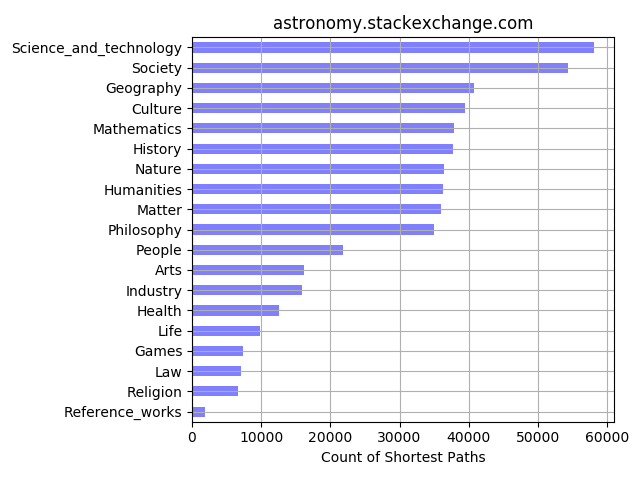
\includegraphics[width=1\linewidth]{imgs/path-counts/astronomy_stackexchange_com}
        \caption{Paths count for Astronomy}
        \label{fig:path-count-astronomy}
    \end{subfigure}%
    \begin{subfigure}{0.5\textwidth}
    \centering
        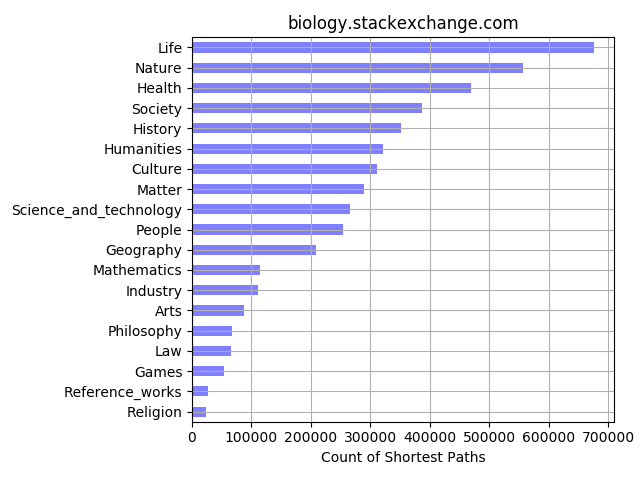
\includegraphics[width=1\linewidth]{imgs/path-counts/biology_stackexchange_com}
        \caption{Paths count for Biology}
        \label{fig:path-count-biology}
    \end{subfigure}
 
     \begin{subfigure}{0.5\textwidth}
    \centering
        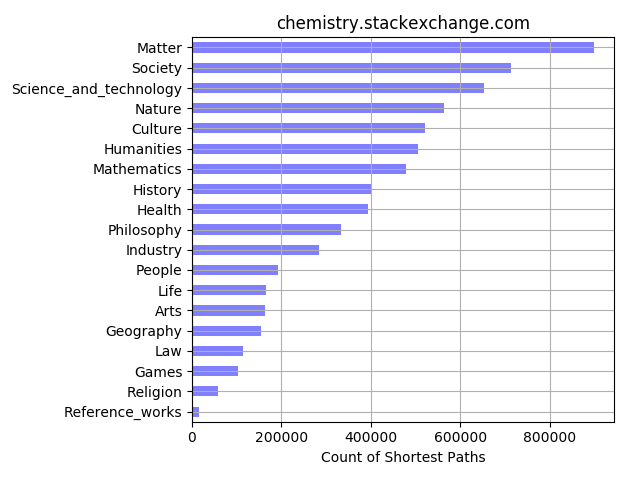
\includegraphics[width=1\linewidth]{imgs/path-counts/chemistry_stackexchange_com}
        \caption{Paths count for Chemistry}
        \label{fig:path-count-chemistry}
    \end{subfigure}%
    \begin{subfigure}{0.5\textwidth}
    \centering
        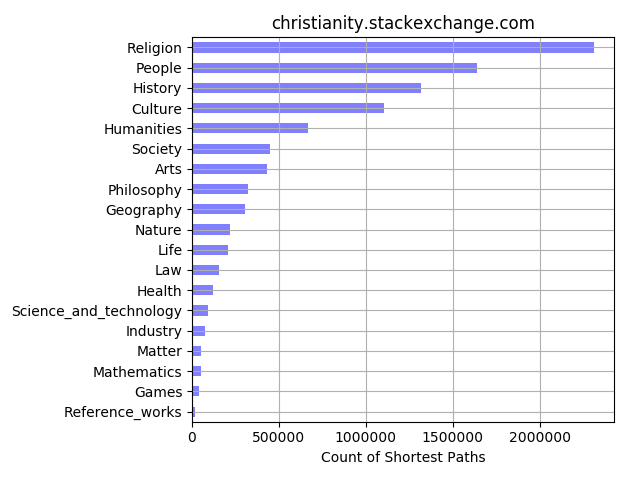
\includegraphics[width=1\linewidth]{imgs/path-counts/christianity_stackexchange_com}
        \caption{Paths count for Christianity}
        \label{fig:path-count-christianity}
    \end{subfigure}

        
     \begin{subfigure}{0.5\textwidth}
    \centering
        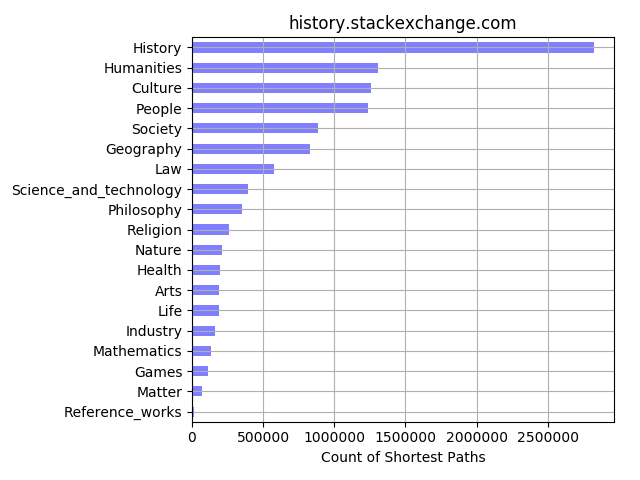
\includegraphics[width=1\linewidth]{imgs/path-counts/history_stackexchange_com}
        \caption{Paths count for History}
        \label{fig:path-count-history}
    \end{subfigure}%
    \begin{subfigure}{0.5\textwidth}
    \centering
        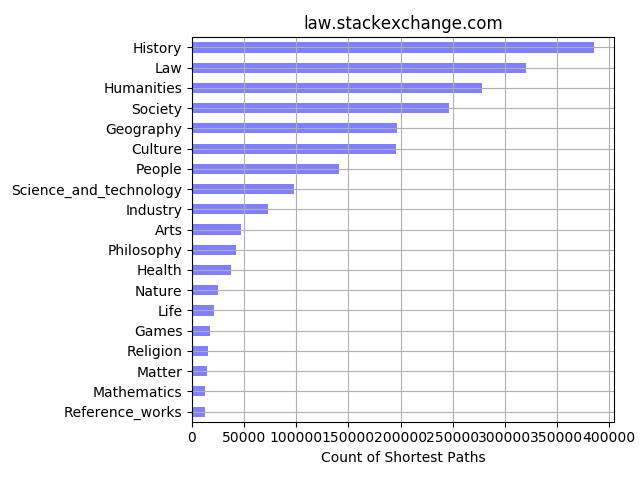
\includegraphics[width=1\linewidth]{imgs/path-counts/law_stackexchange_com}
        \caption{Paths count for Law}
        \label{fig:path-count-law}
    \end{subfigure} 

    \end{figure}
    
 \begin{figure}[H]
 \ContinuedFloat
    \centering
    \begin{subfigure}{0.5\textwidth}
    \centering
        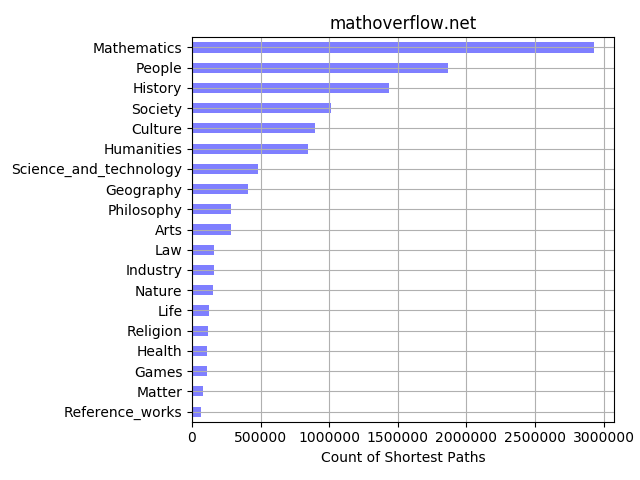
\includegraphics[width=1\linewidth]{imgs/path-counts/mathoverflow_net}
        \caption{Paths count for Math}
        \label{fig:path-count-math}
    \end{subfigure}%
    \begin{subfigure}{0.5\textwidth}
    \centering
        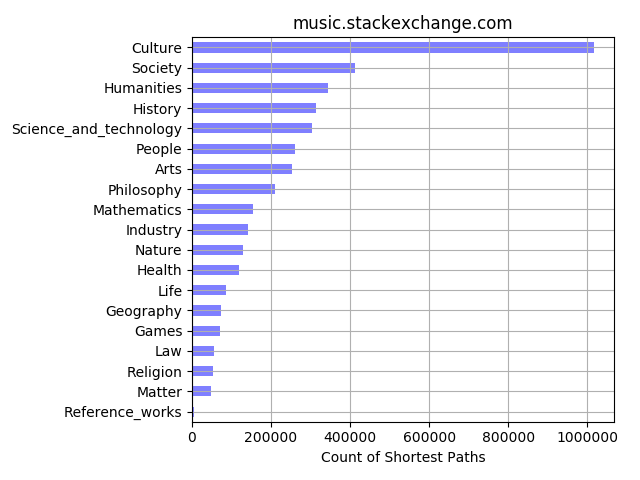
\includegraphics[width=1\linewidth]{imgs/path-counts/music_stackexchange_com}
        \caption{Paths count for Music}
        \label{fig:path-count-music}
    \end{subfigure}
 
     \begin{subfigure}{0.5\textwidth}
    \centering
        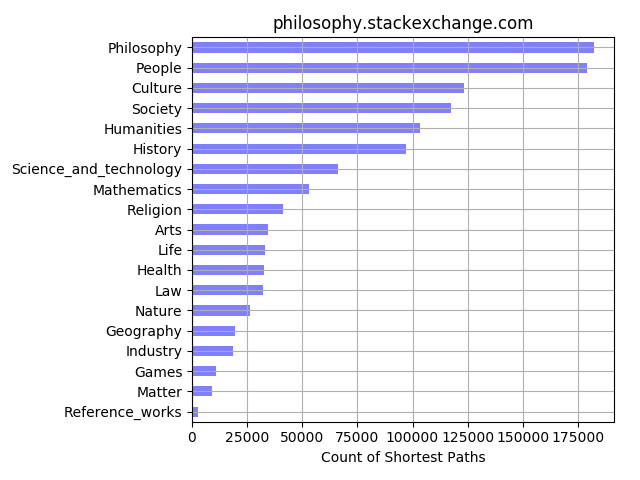
\includegraphics[width=1\linewidth]{imgs/path-counts/philosophy_stackexchange_com}
        \caption{Paths count for Philosophy}
        \label{fig:path-count-philosophy}
    \end{subfigure}%
    \begin{subfigure}{0.5\textwidth}
    \centering
        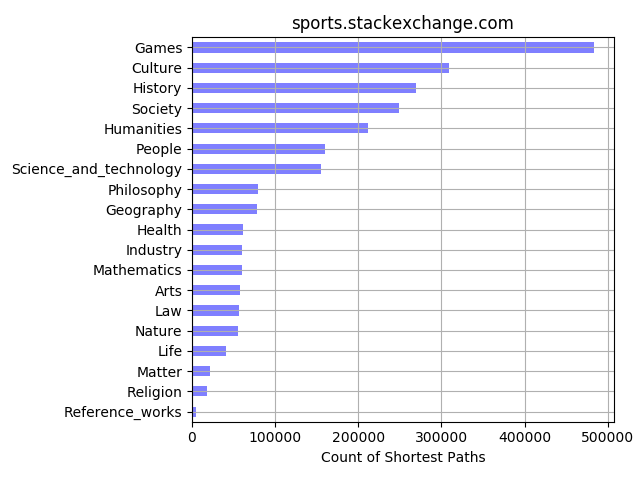
\includegraphics[width=1\linewidth]{imgs/path-counts/sports_stackexchange_com}
        \caption{Paths count for Sports}
        \label{fig:path-count-sports}
    \end{subfigure}
   
 
    \caption{The number of shortest paths through the proposed method. The X-axis shows the number of paths found for each top-level category (displayed on the Y-axis) }
    \label{fig:complete-path-count-distribution}
    
\end{figure}

\begin{figure}[H]
    \centering
	\begin{subfigure}{0.9\textwidth}
    	\centering
        	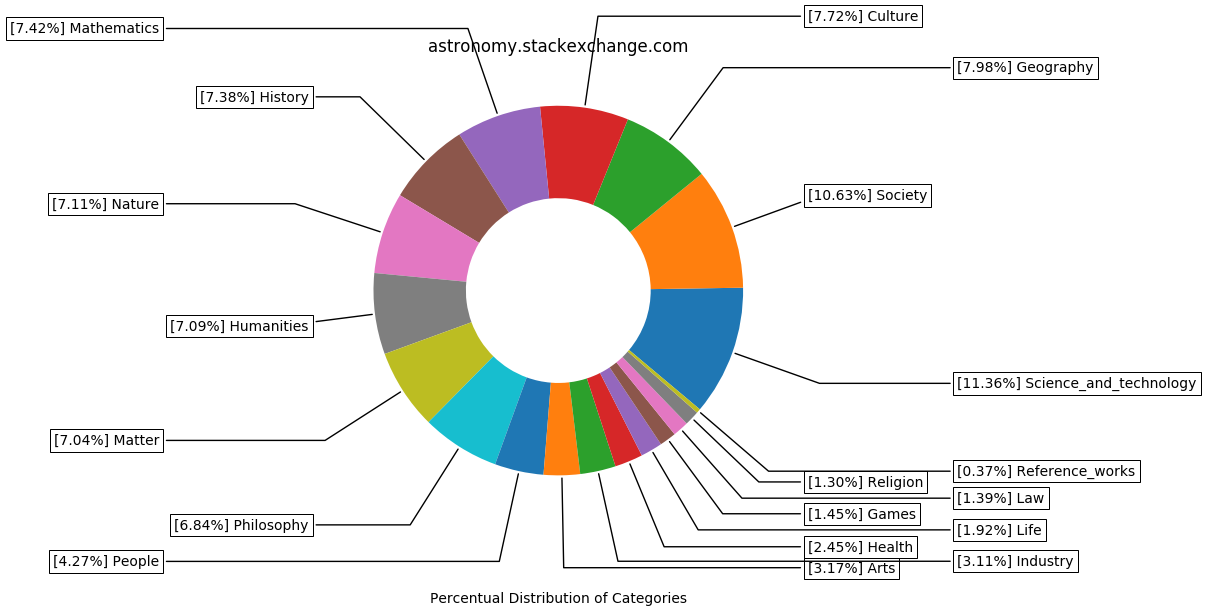
\includegraphics[width=1\linewidth]{imgs/percentual-distribution/astronomy_stackexchange_com_donut}
        	\caption{Percentage distribution of categories for Astronomy}
        	\label{fig:percentage-distribution-astronomy}
    \end{subfigure}%
    
\par\bigskip % 
\par\bigskip % 
	\begin{subfigure}{0.9\textwidth}
    \centering
        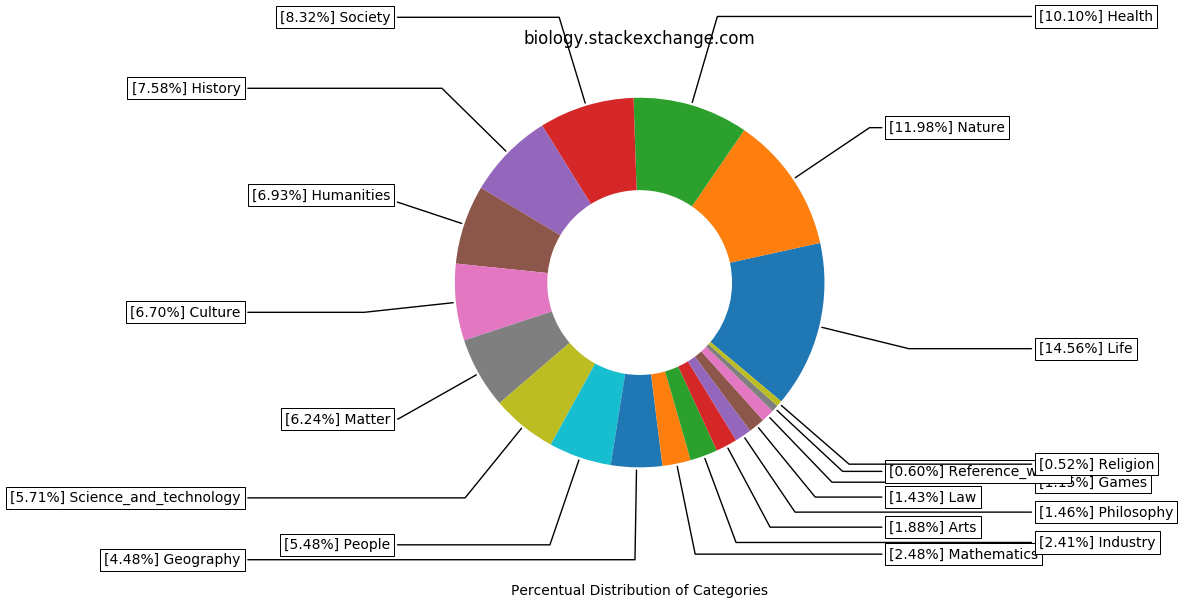
\includegraphics[width=1\linewidth]{imgs/percentual-distribution/biology_stackexchange_com_donut}
        \caption{Percentage distribution of categories for Biology}
        \label{fig:percentage-distribution-biology}
    \end{subfigure}
 
\par\bigskip % 
\par\bigskip % 

	\begin{subfigure}{0.9\textwidth}
    \centering
    	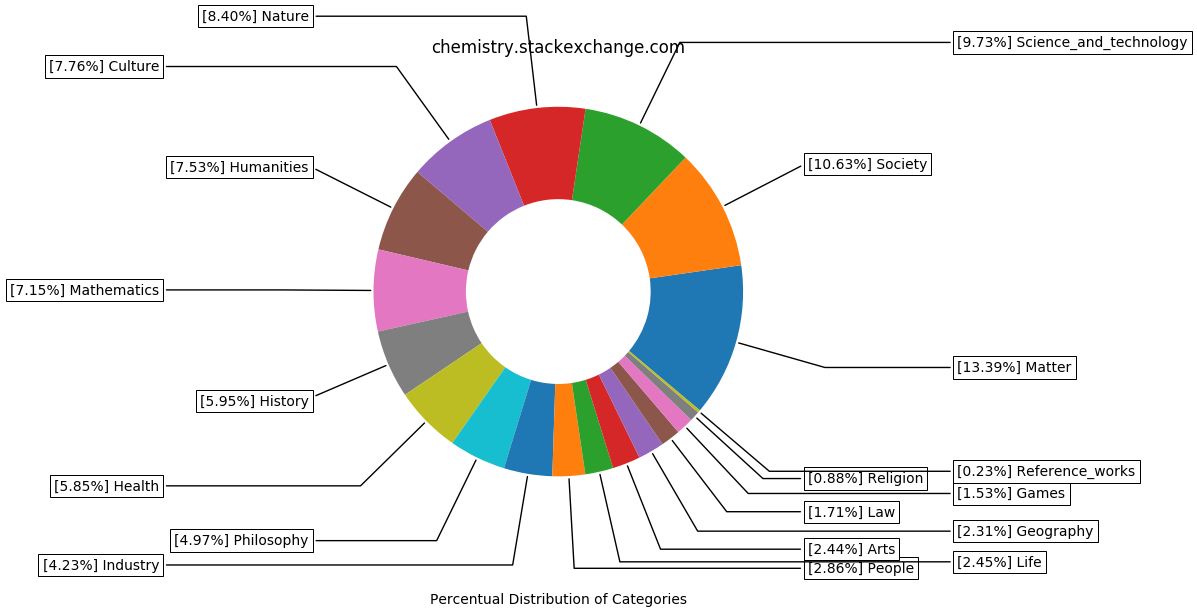
\includegraphics[width=1\linewidth]{imgs/percentual-distribution/chemistry_stackexchange_com_donut}
        \caption{Percentage distribution of categories for Chemistry}
        \label{fig:percentage-distribution-chemistry}
    \end{subfigure}%
\end{figure}
    

\begin{figure}[H]
\ContinuedFloat
\begin{subfigure}{0.9\textwidth}
    \centering
        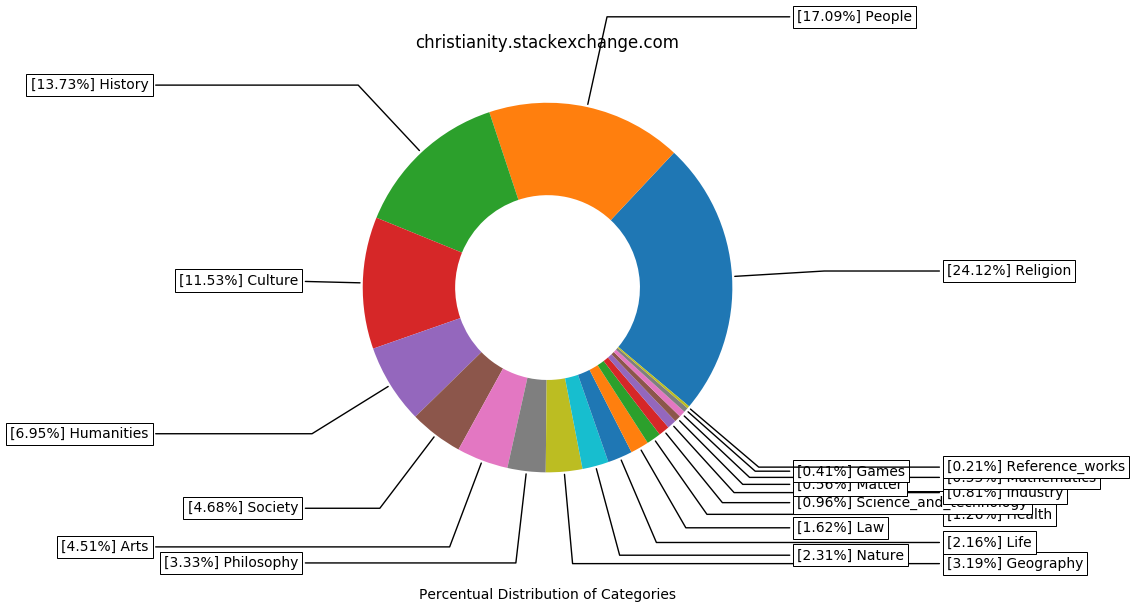
\includegraphics[width=1\linewidth]{imgs/percentual-distribution/christianity_stackexchange_com_donut}
        \caption{Percentage distribution of categories Christianity}
        \label{fig:percentage-distribution-christianity}
    \end{subfigure}
    
     	\par\bigskip % 
    \par\bigskip % 
        
     \begin{subfigure}{0.9\textwidth}
    \centering
        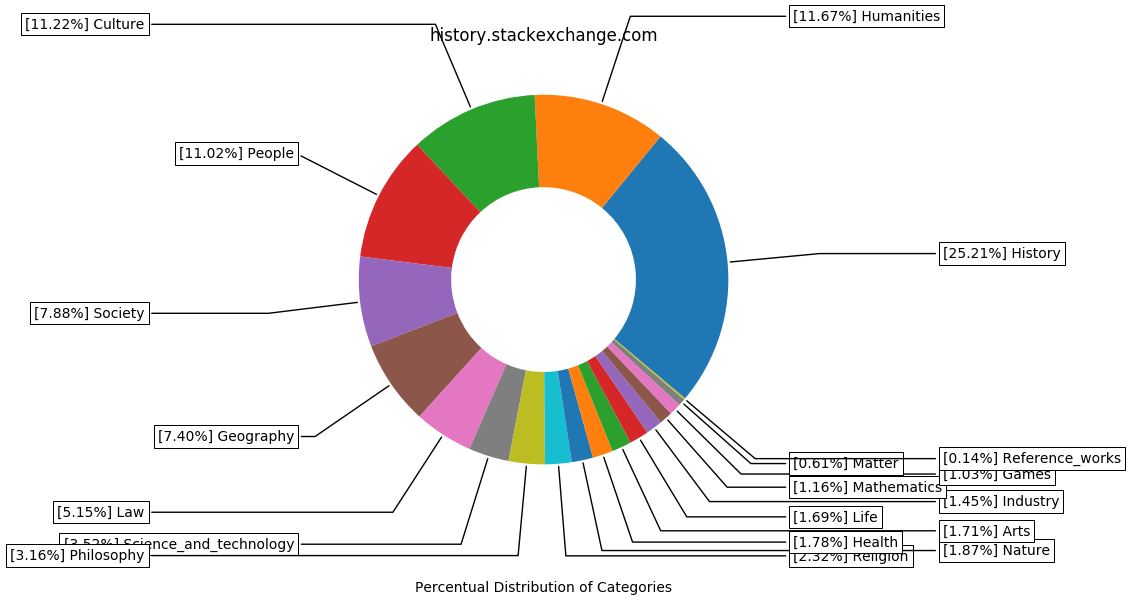
\includegraphics[width=1\linewidth]{imgs/percentual-distribution/history_stackexchange_com_donut}
        \caption{Percentage distribution of categories for History}
        \label{fig:percentage-distribution-history}
    \end{subfigure}%
    
     \par\bigskip % 
    \par\bigskip % 
    \begin{subfigure}{0.9\textwidth}
    \centering
        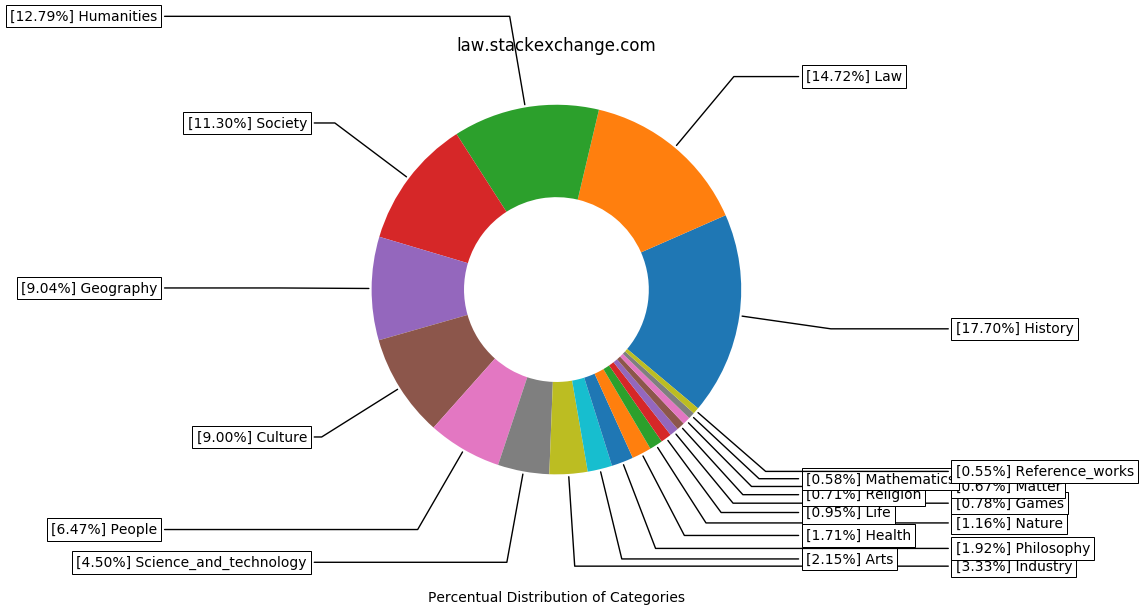
\includegraphics[width=1\linewidth]{imgs/percentual-distribution/law_stackexchange_com_donut}
        \caption{Percentage distribution of categories for Law}
        \label{fig:percentage-distribution-law}
    \end{subfigure} 
 \end{figure}
 
 
\begin{figure}[H]
\ContinuedFloat

    \begin{subfigure}{0.9\textwidth}
    \centering
        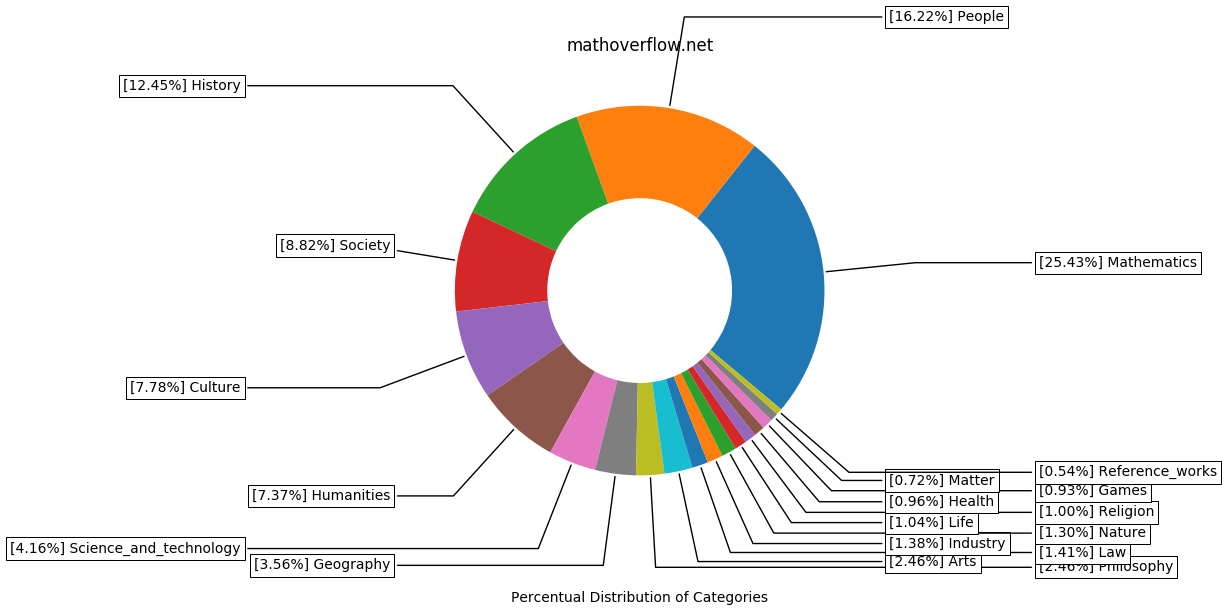
\includegraphics[width=1\linewidth]{imgs/percentual-distribution/mathoverflow_net_donut}
        \caption{Percentage distribution of categories for Math}
        \label{fig:percentage-distribution-math}
    \end{subfigure}%
    
    \begin{subfigure}{0.9\textwidth}
    \centering
        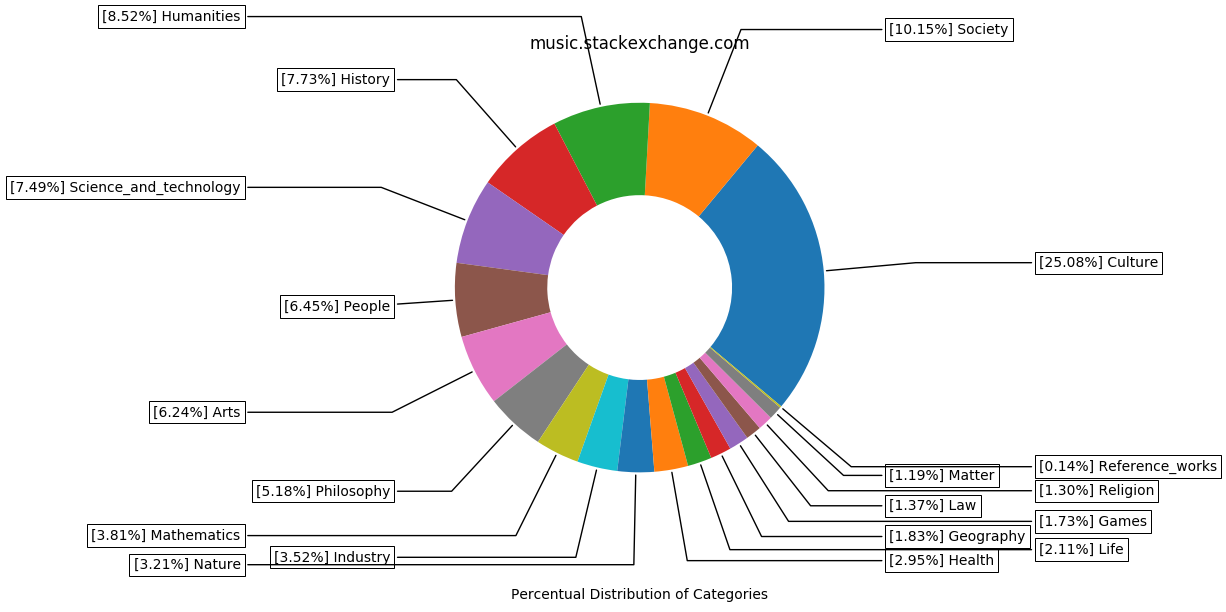
\includegraphics[width=1\linewidth]{imgs/percentual-distribution/music_stackexchange_com_donut}
        \caption{Percentage distribution of categories for Music}
        \label{fig:percentage-distribution-music}
    \end{subfigure}
 
     \begin{subfigure}{0.9\textwidth}
    \centering
        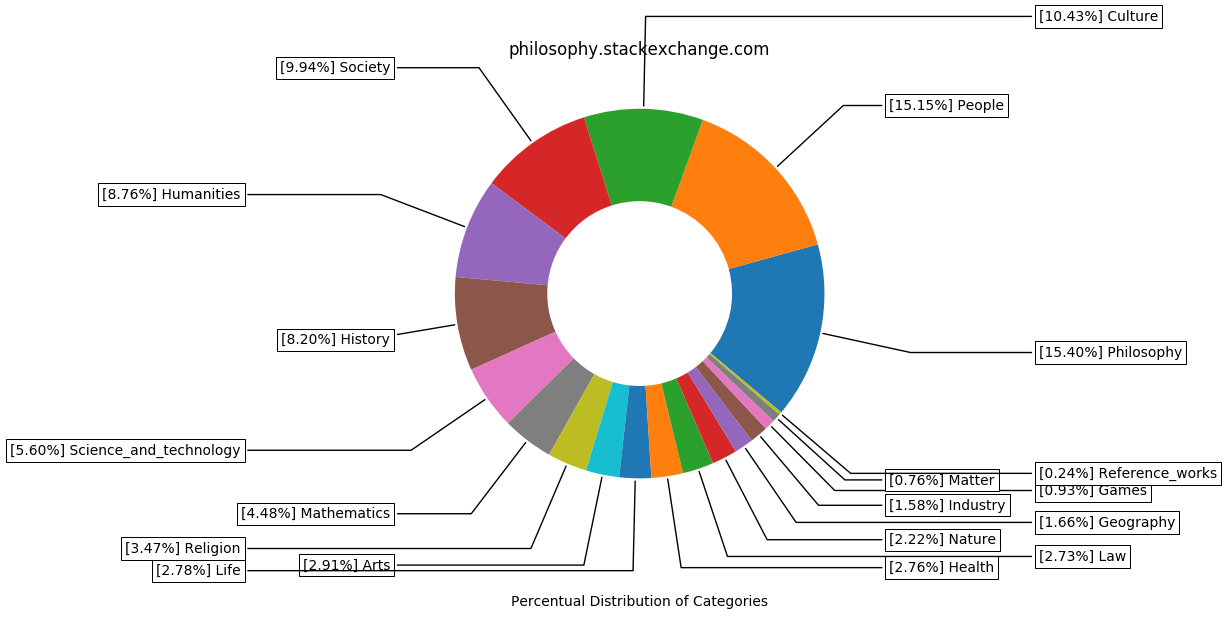
\includegraphics[width=1\linewidth]{imgs/percentual-distribution/philosophy_stackexchange_com_donut}
        \caption{Percentage distribution of categories for Philosophy}
        \label{fig:percentage-distribution-philosophy}
    \end{subfigure}%
 
\end{figure}
 
  
\begin{figure}[H]
\ContinuedFloat

    \begin{subfigure}{0.9\textwidth}
    \centering
        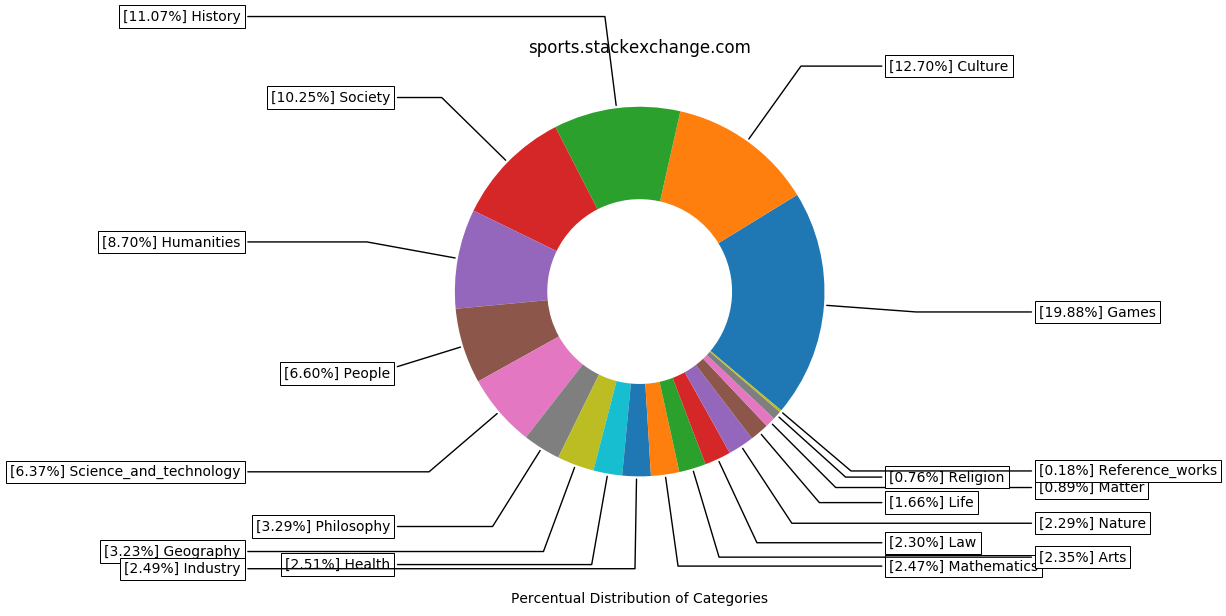
\includegraphics[width=1\linewidth]{imgs/percentual-distribution/sports_stackexchange_com_donut}
        \caption{Percentage distribution of categories for Sports}
        \label{fig:path-sports}
    \end{subfigure}
   
 
    \caption{Percentage distribution of categories for each of the communities evaluated according to the proposed method. }
    \label{fig:complete-percentage-distribution}
    
\end{figure}


\section{\hspace*{3pt} Crowd}

In order to verify if the classification generated by the proposed method is coherent for real users, we conducted an experiment with human judges in order to verify how much they agree with the automatic classification result. For this purpose, we use the stack exchange datasets to make the comparison possible with the experiment described in section \ref{section:proof-of-concept}.



\subsection{\hspace*{3pt} Experimental Design}

Due to the accessibility of established micro-task crowd-sourcing platforms such as Amazon’s Mechanical Turk\footnote{\url{www.mturk.com}} and CrowdFlower, researchers are actively turning toward paid crowd-sourcing to solve data-centric tasks that require human input, such as building ground truths, validating results, and curating data \cite{7156008}.

We used CrowdFlower\footnote{\url{http://crowdflower.com}}, an on-line platform which provides access to a workforce to perform tasks.  It automatically allocates the available tasks to contributors and tests them against known answers, named Gold Standard. Their performance on test questions indicates how much the system trusts each contributor and if they become untrusted, they are removed from the task, and the work is discarded.

For this experiment, we also considered as top-level categories the ones defined as Main topic classifications on Wikipedia (19 categories by the date of data extraction). 

For each one of the ten communities, we run the experiment with 200 different random items extracted from the stack exchange dataset. 

We asked each contributor to read texts randomly chosen from the dataset and answer to what extent the text belongs to each one of the categories on a scale ranging from 0 (not at all) to 3 (to a great extent). 

To alleviate the intensive task of judging for 19 Categories, we asked the participants the evaluate the top-3 categories with greatest percentage distribution and two other random categories.  Figure \ref{fig:example-question} shows a real example of task delivered to contributors for the dataset Biology. The categories LIFE, HEALTH and NATURE are the top-3 categories with the highest degree of membership according to our method (see figures \ref{fig:path-count-biology} and \ref{fig:percentage-distribution-biology}). The categories RELIGION and GAMES were randomly introduced in the survey. 

Random categories were included to validate whether, in addition to agreeing with the categories that appear with the highest distribution in the classification, they also agree with those that do not belong to the most prominent categories.  

Moreover, this mechanism reinforces the verification of the validity of the judgments, since random categories cannot have a distribution of responses similar to those in the top-3 categories.




\begin{figure}[!h]
\centering
  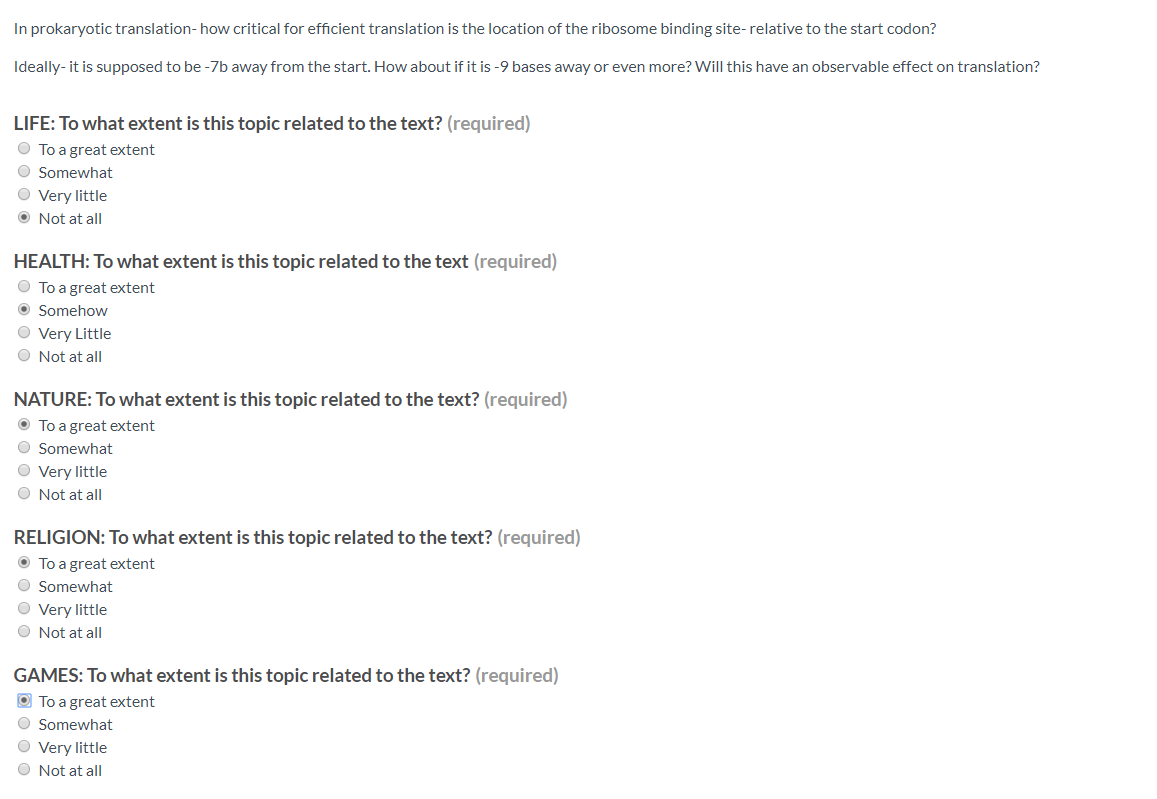
\includegraphics[width=\linewidth]{question-example}
  \caption{Example of task delivered to contributors in the dataset Biology}
  \label{fig:example-question}
\end{figure}

 
To select the participants able to perform the task proposed in the experiment, we created a series of 30 test questions for the stack exchange dataset, so that the participates with low performance in the test questions were eliminated in this stage.


As described in \cite{Gadiraju:2017}, many research works have referred to the importance of task clarity tangentially and stressed the positive impact of task design, clear instructions and descriptions on the quality of crowdsourced work. 

In this regard, we provided a detailed guide for contributors to make sure they clearly understand how to perform the task, with examples of good and bad judgments and also with a description of each one of the 19 categories. To make sure the task is perfectly designed, CrowdFlower platform offers a consulting service where the top-rated contributors evaluate and give feedback on the quality of a given task. An example of the feedback given by this consulting service can be seen in figure \ref{fig:example-feedback}. 

We adjusted the task description according to the suggestions in the feedback by providing more and contextualized examples, as well as explaining, for each test question, the reason why the alternatives were considered wrong or correct.  

\begin{figure}[!h]
\centering
  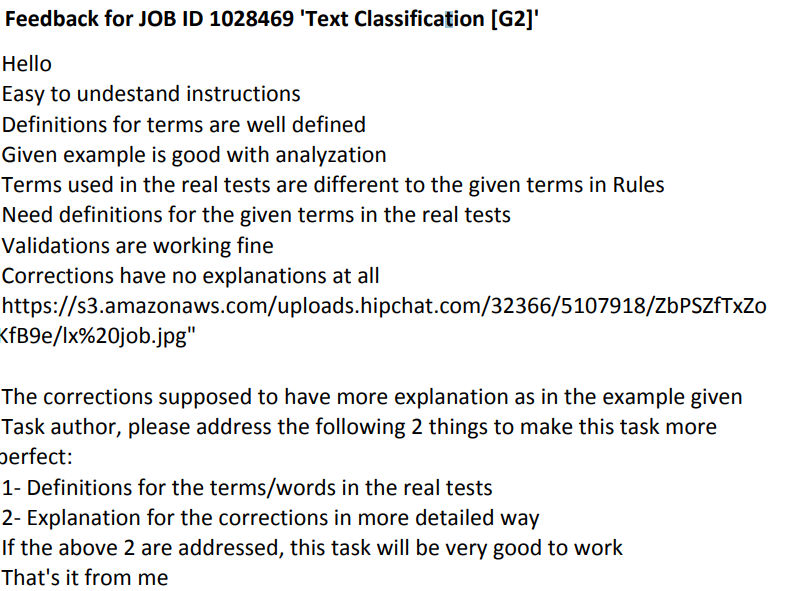
\includegraphics[width=\linewidth]{crowd-feedback}
  \caption{Example of feedback given by the consulting service provided by CrowdFlower platform}
  \label{fig:example-feedback}
\end{figure}


in the final experiment, 1265 unique contributors participated from June to August of 2018. The overall setup for the experiment is presented in table \ref{tab:experiment-overview}. A trusted judgment is an answer from a contributor with an accuracy score higher than the minimum accuracy considered for this experiment (0.75), while an untrusted judgment is an answer from a contributor whose accuracy score has fallen below this value.

\begin{table}[!h]

\centering
\caption{Overall setup for the experiment with crowd workers}
\label{tab:experiment-overview}
\resizebox{\textwidth}{!}{%
\begin{tabular}{@{}llllll@{}}
\toprule
Community         & Trusted Judgments & Untrusted Judgments & Average Judgments per Row & Average Trust of Workers & Unique Workers \\ \midrule
Astronomy         & 640               & 36                  & 3.2000                    & 0.8651                   & 128            \\
Biology (Elite)   & 612               & 48                  & 3.0600                    & 0.8390                   & 122            \\
Biology (Regular) & 1040              & 278                 & 5.2000                    & 0.8366                   & 208            \\
Chemistry         & 751               & 12                  & 3.7550                    & 0.8197                   & 150            \\
Christianity      & 628               & 16                  & 3.1558                    & 0.8843                   & 125            \\
History           & 602               & 76                  & 3.0251                    & 0.7997                   & 120            \\
Law               & 601               & 0                   & 3.0050                    & 0.8831                   & 120            \\
Math              & 630               & 32                  & 3.1500                    & 0.9306                   & 126            \\
Music             & 602               & 28                  & 3.0100                    & 0.9137                   & 120            \\
Philosophy        & 717               & 108                 & 3.5850                    & 0.8376                   & 143            \\
Sports            & 629               & 32                  & 3.1608                    & 0.8349                   & 125            \\ \bottomrule
\end{tabular}%
}
\end{table}

\subsection{\hspace*{3pt} Elite Contributors X Regular Contributors}

Before we run the experiment with all ten communities, we first evaluated whether there is a difference between the quality of judgments performed by elite contributors and the judgments made by regular contributors. The elite contributors (also called level-3 contributors in the context of CrowdFlower platform) are those who completed over 100 test questions across hundreds of different types of tasks and have a near perfect overall accuracy. To perform this verification, we ran the experiment using the Biology dataset in two different groups: one only with regular contributors and the other with level-3 contributors. They were asked to judge the same set of 200 questions. 

A statistical test was applied aiming at determining if the results obtained in the answers given by the two groups can be considered significantly different from each other. The Wilcoxon-Mann-Whitney nonparametric statistical inference test was applied\cite{feltovich2003nonparametric}. This test compares the mean of two independent samples and does not require normality and homoscedasticity in the series of values compared. The level of significance was set at 95\%. The p-value evaluates the result of this statistical test. The lower is the p-value, the higher the significance of the outcome. For a significance level of 95\%, if the p-value is smaller than 0.05, we can conclude that responses observed for the two groups are distinct. 

We obtained a p-value of  0.267, meaning that there is no significant difference between the answers given by the two groups. 

If we analyze the table \ref{tab:experiment-overview} it is possible to see that regular users are less efficient and thus more judgments are needed to achieve a reasonable level of agreement. 

Even though the price paid to regular contributors is lower in comparison to elite contributors, we decided to admit only level-3 users.

\subsection{\hspace*{3pt} Quality Control}

While dealing with a random collection of strangers to perform relevance evaluation, two primary concerns have risen:  i) How to ensure that contributors performing the evaluation will have the necessary skill or knowledge? ii) How to make sure that the contributors will make a high-quality effort to do the work, rather than clicking randomly on the responses?

 
To address these questions, we defined some parameters of quality regarding the contributors and the experiment:

\begin{enumerate}

\item We restricted the participation to contributors from English-speaking countries to ensure that they understood the task and instructions adequately. 

\item We restricted the participation to Level-3 contributors on CrowdFlower, meaning that only those who completed over 100 test questions across hundreds of different types of tasks and have a near perfect overall accuracy. They are contributors of the highest quality on CrowdFlower.

\item We restricted each contributor to a maximum of five judgments across all datasets, to minimize the number of contributors trying to complete a massive number of tasks in order to make more money 

\item We predefined the minimum of 0.75 regarding the level of agreement among the contributors for each row of text evaluated. In case a row does not reach this value with the default number of 3 judgments, new judgments were requested until the agreement coefficient reached 0.75.

\end{enumerate}

\subsection{\hspace*{3pt} Results and Discussion}



 \begin{figure}[H]
    \centering
    \begin{subfigure}{0.5\textwidth}
    \centering
        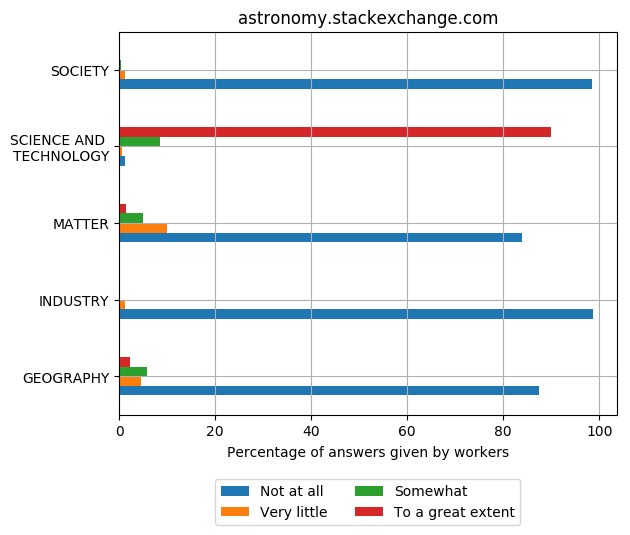
\includegraphics[width=1\linewidth]{imgs/crowd-results/astronomy_stackexchange_com}
        \caption{Distribution of Answers for Astronomy}
        \label{fig:crowd-results-astronomy}
    \end{subfigure}%
    \begin{subfigure}{0.5\textwidth}
    \centering
        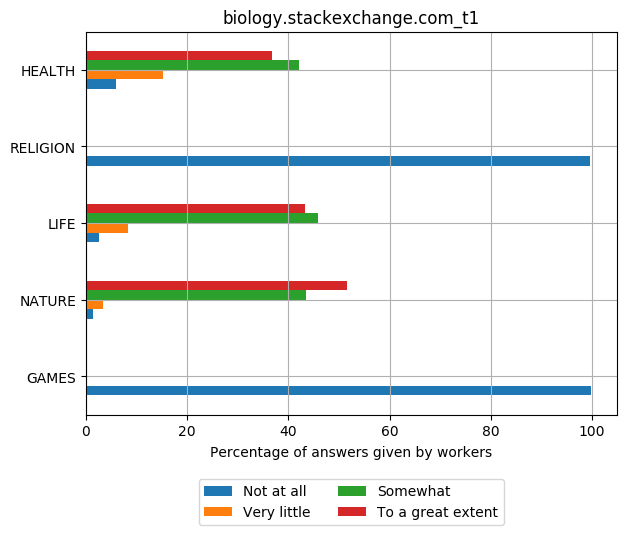
\includegraphics[width=1\linewidth]{imgs/crowd-results/biology_stackexchange_com_t1}
        \caption{Distribution of Answers for Biology (Regular)}
        \label{fig:crowd-results-biology-1}
    \end{subfigure}
 
     \begin{subfigure}{0.5\textwidth}
    \centering
        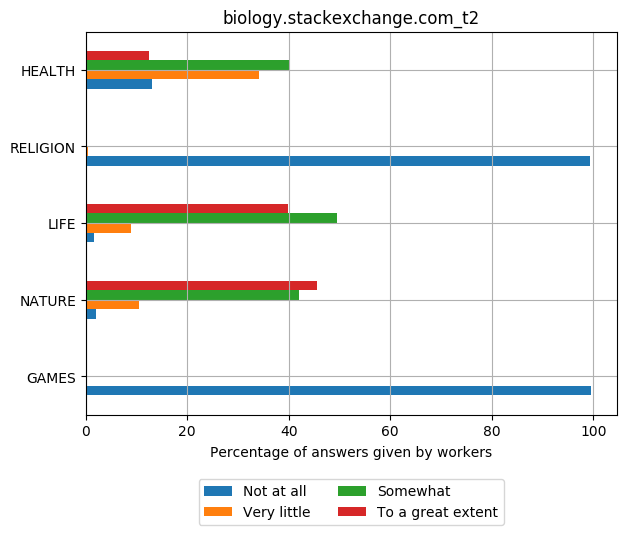
\includegraphics[width=1\linewidth]{imgs/crowd-results/biology_stackexchange_com_t2}
        \caption{Distribution of Answers for Biology (Elite)}
        \label{fig:crowd-results-biology-2}
    \end{subfigure}%
    \begin{subfigure}{0.5\textwidth}
    \centering
        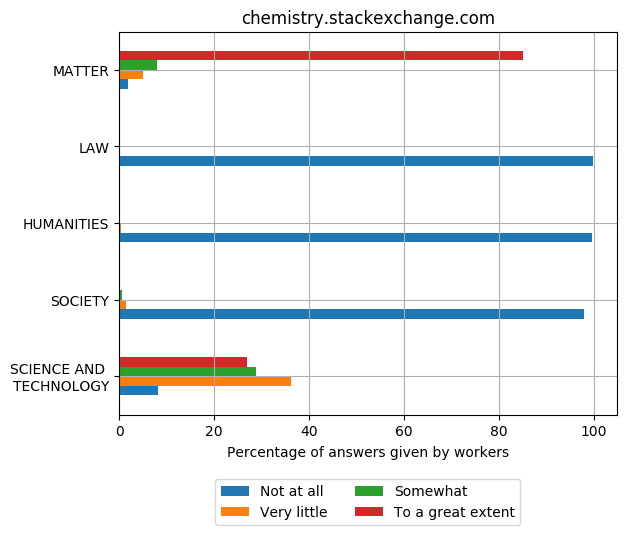
\includegraphics[width=1\linewidth]{imgs/crowd-results/chemistry_stackexchange_com}
        \caption{Distribution of Answers for Chemistry}
        \label{fig:crowd-results-chemistry}
    \end{subfigure}

        
     \begin{subfigure}{0.5\textwidth}
    \centering
        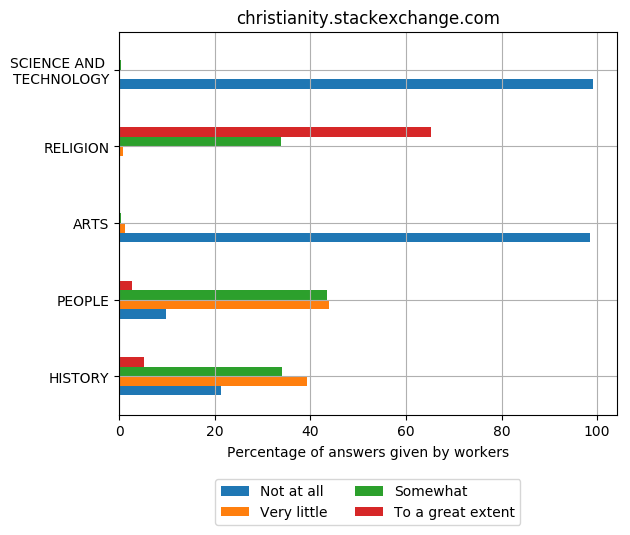
\includegraphics[width=1\linewidth]{imgs/crowd-results/christianity_stackexchange_com}
        \caption{Distribution of Answers for Christianity}
        \label{fig:crowd-results-christianity}
    \end{subfigure}%
    \begin{subfigure}{0.5\textwidth}
    \centering
        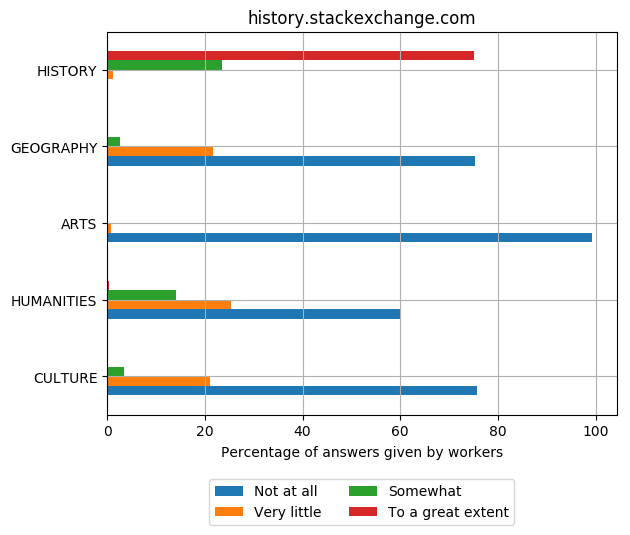
\includegraphics[width=1\linewidth]{imgs/crowd-results/history_stackexchange_com}
        \caption {Distribution of Answers for  History}
        \label{fig:crowd-results-history}
    \end{subfigure} 

    \end{figure}
    
 \begin{figure}[H]
 \ContinuedFloat
    \centering
    \begin{subfigure}{0.5\textwidth}
    \centering
        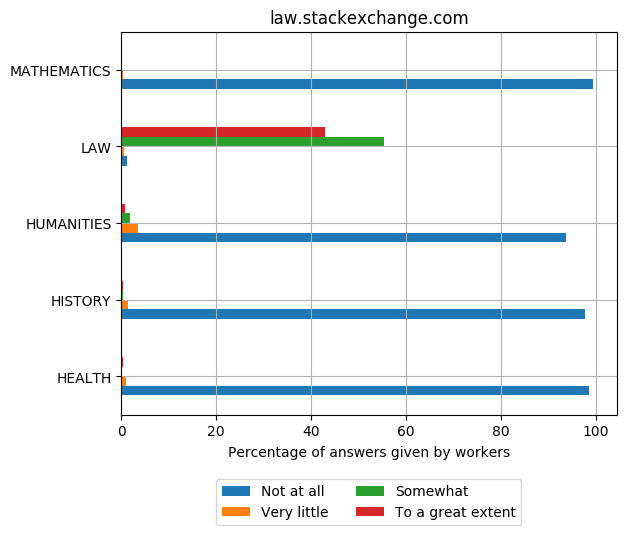
\includegraphics[width=1\linewidth]{imgs/crowd-results/law_stackexchange_com}
        \caption{Distribution of Answers for Law}
        \label{fig:crowd-results-law}
    \end{subfigure}%
    \begin{subfigure}{0.5\textwidth}
    \centering
        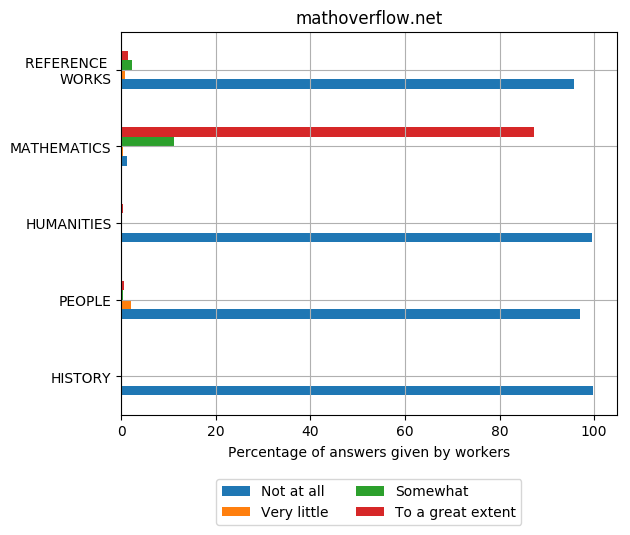
\includegraphics[width=1\linewidth]{imgs/crowd-results/mathoverflow_net}
        \caption{Distribution of Answers for Math}
        \label{fig:crowd-results-math}
    \end{subfigure}
 
     \begin{subfigure}{0.5\textwidth}
    \centering
        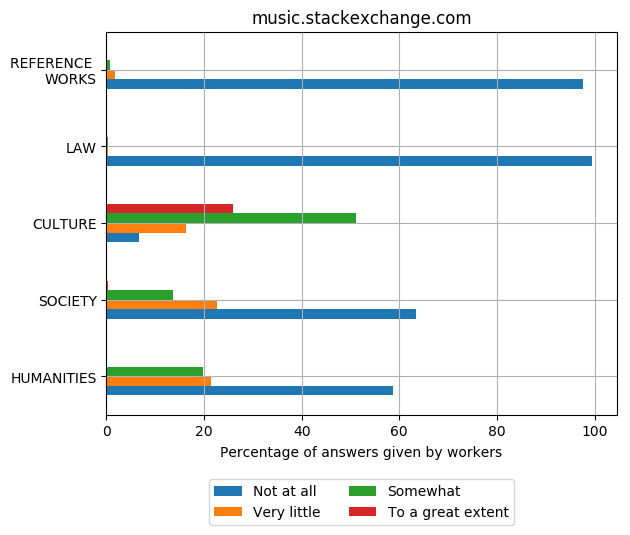
\includegraphics[width=1\linewidth]{imgs/crowd-results/music_stackexchange_com}
        \caption{Distribution of Answers for Music}
        \label{fig:crowd-results-music}
    \end{subfigure}%
    \begin{subfigure}{0.5\textwidth}
    \centering
        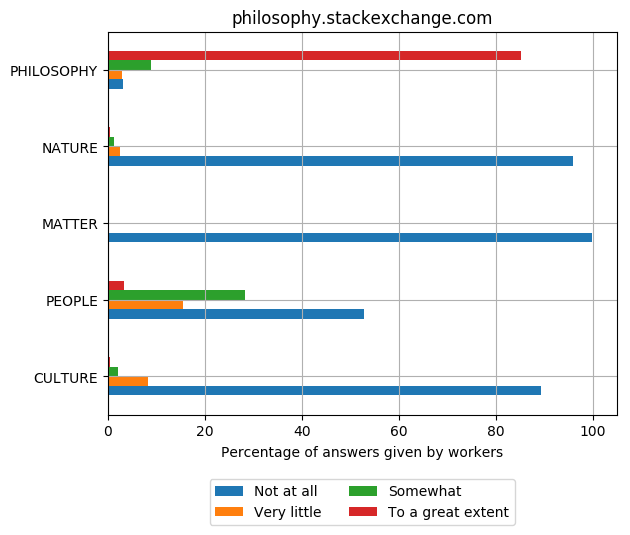
\includegraphics[width=1\linewidth]{imgs/crowd-results/philosophy_stackexchange_com}
        \caption{Distribution of Answers for Philosophy}
        \label{fig:crowd-results-philosophy}
    \end{subfigure}
    
     \begin{subfigure}{0.5\textwidth}
    \centering
        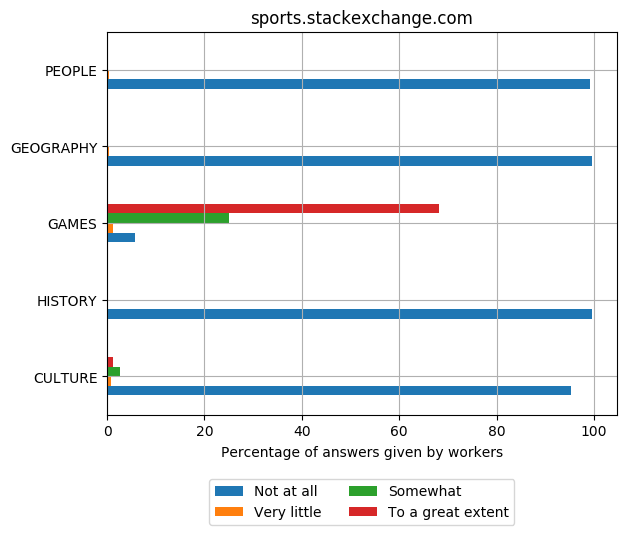
\includegraphics[width=1\linewidth]{imgs/crowd-results/sports_stackexchange_com}
        \caption{Distribution of Answers for Sports}
        \label{fig:crowd-results-sports}
    \end{subfigure}%
 \caption{Percentage distribution of answers given by crowd contributors for each one of the ten communities evaluated }
    \label{fig:complete-crowd-distribution}
    
\end{figure}

